% Created by tikzDevice version 0.12.3.1 on 2021-12-04 14:20:28
% !TEX encoding = UTF-8 Unicode
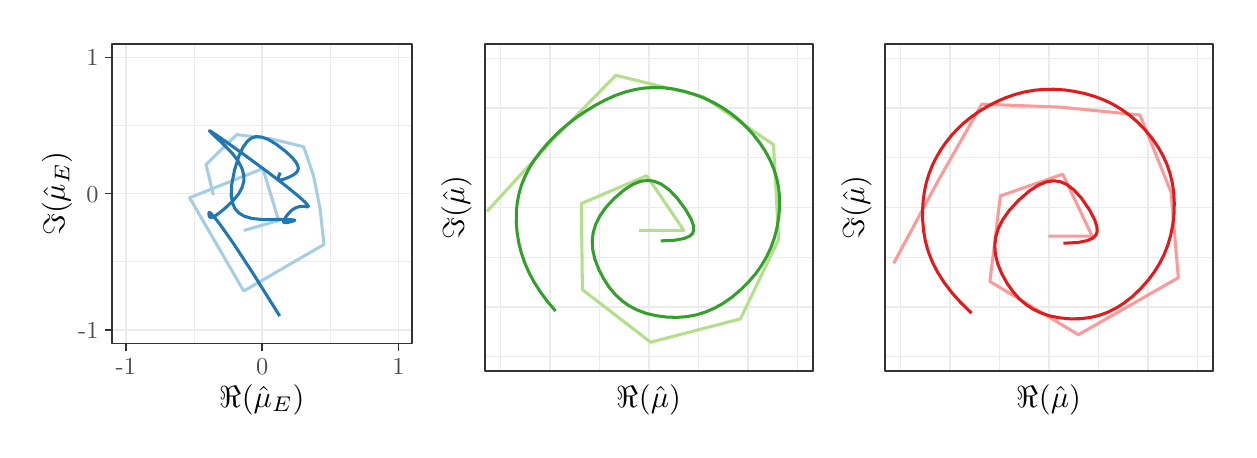
\begin{tikzpicture}[x=1pt,y=1pt]
\definecolor{fillColor}{RGB}{255,255,255}
\begin{scope}
\definecolor{drawColor}{RGB}{255,255,255}
\definecolor{fillColor}{RGB}{255,255,255}

\path[draw=drawColor,line width= 0.6pt,line join=round,line cap=round,fill=fillColor] (  0.22,  0.00) rectangle (144.32,144.54);
\end{scope}
\begin{scope}
\definecolor{fillColor}{RGB}{255,255,255}

\path[fill=fillColor] ( 30.47, 30.69) rectangle (138.82,139.04);
\definecolor{drawColor}{gray}{0.92}

\path[draw=drawColor,line width= 0.3pt,line join=round] ( 30.47, 60.24) --
	(138.82, 60.24);

\path[draw=drawColor,line width= 0.3pt,line join=round] ( 30.47,109.49) --
	(138.82,109.49);

\path[draw=drawColor,line width= 0.3pt,line join=round] ( 60.02, 30.69) --
	( 60.02,139.04);

\path[draw=drawColor,line width= 0.3pt,line join=round] (109.27, 30.69) --
	(109.27,139.04);

\path[draw=drawColor,line width= 0.6pt,line join=round] ( 30.47, 35.61) --
	(138.82, 35.61);

\path[draw=drawColor,line width= 0.6pt,line join=round] ( 30.47, 84.86) --
	(138.82, 84.86);

\path[draw=drawColor,line width= 0.6pt,line join=round] ( 30.47,134.11) --
	(138.82,134.11);

\path[draw=drawColor,line width= 0.6pt,line join=round] ( 35.39, 30.69) --
	( 35.39,139.04);

\path[draw=drawColor,line width= 0.6pt,line join=round] ( 84.64, 30.69) --
	( 84.64,139.04);

\path[draw=drawColor,line width= 0.6pt,line join=round] (133.89, 30.69) --
	(133.89,139.04);
\definecolor{drawColor}{RGB}{166,206,227}

\path[draw=drawColor,line width= 1.1pt,line join=round] ( 78.02, 71.57) --
	( 90.60, 75.15) --
	( 84.91, 93.95) --
	( 58.45, 83.39) --
	( 77.98, 49.69) --
	(106.99, 66.49) --
	(105.59, 79.32) --
	(103.21, 91.32) --
	( 99.66,101.81) --
	( 88.12,104.61) --
	( 75.44,106.20) --
	( 64.37, 95.38) --
	( 67.01, 84.35);
\definecolor{drawColor}{RGB}{31,120,180}

\path[draw=drawColor,line width= 1.1pt,line join=round] ( 91.17, 92.47) --
	( 90.67, 91.26) --
	( 90.49, 90.53) --
	( 90.51, 90.13) --
	( 90.64, 89.93) --
	( 90.91, 89.82) --
	( 91.45, 89.84) --
	( 92.41, 90.07) --
	( 93.94, 90.65) --
	( 95.81, 91.55) --
	( 96.95, 92.41) --
	( 97.53, 93.21) --
	( 97.71, 94.02) --
	( 97.53, 94.98) --
	( 96.86, 96.24) --
	( 95.49, 97.92) --
	( 93.14,100.11) --
	( 89.68,102.77) --
	( 86.60,104.58) --
	( 84.23,105.38) --
	( 82.37,105.46) --
	( 80.79,104.95) --
	( 79.30,103.79) --
	( 77.78,101.72) --
	( 76.22, 98.39) --
	( 74.67, 93.41) --
	( 73.66, 88.22) --
	( 73.47, 84.36) --
	( 73.90, 81.54) --
	( 74.82, 79.47) --
	( 76.20, 77.91) --
	( 78.20, 76.71) --
	( 81.06, 75.87) --
	( 85.10, 75.47) --
	( 89.86, 75.52) --
	( 93.13, 75.51) --
	( 95.07, 75.44) --
	( 96.03, 75.35) --
	( 96.36, 75.28) --
	( 96.40, 75.23) --
	( 96.28, 75.15) --
	( 95.75, 74.94) --
	( 94.53, 74.60) --
	( 93.51, 74.40) --
	( 92.90, 74.37) --
	( 92.58, 74.44) --
	( 92.44, 74.56) --
	( 92.40, 74.75) --
	( 92.47, 75.10) --
	( 92.76, 75.71) --
	( 93.36, 76.67) --
	( 94.17, 77.70) --
	( 94.96, 78.52) --
	( 95.75, 79.16) --
	( 96.55, 79.64) --
	( 97.38, 79.97) --
	( 98.24, 80.18) --
	( 99.16, 80.26) --
	(100.16, 80.20) --
	(101.04, 80.09) --
	(101.32, 80.16) --
	(101.34, 80.33) --
	(101.00, 80.86) --
	( 99.89, 82.04) --
	( 97.52, 84.16) --
	( 93.42, 87.50) --
	( 87.12, 92.33) --
	( 78.50, 98.67) --
	( 71.89,103.42) --
	( 68.04,106.08) --
	( 66.22,107.27) --
	( 65.65,107.57) --
	( 65.61,107.56) --
	( 65.90,107.21) --
	( 67.19,105.93) --
	( 70.22,103.13) --
	( 73.70, 99.62) --
	( 76.00, 96.59) --
	( 77.37, 93.95) --
	( 78.00, 91.60) --
	( 78.02, 89.40) --
	( 77.45, 87.20) --
	( 76.21, 84.86) --
	( 74.11, 82.29) --
	( 71.37, 79.71) --
	( 69.26, 77.96) --
	( 67.78, 76.92) --
	( 66.81, 76.41) --
	( 66.21, 76.25) --
	( 65.86, 76.31) --
	( 65.63, 76.52) --
	( 65.46, 77.00) --
	( 65.41, 77.82) --
	( 65.52, 78.08) --
	( 65.92, 77.89) --
	( 67.15, 76.64) --
	( 69.75, 73.32) --
	( 74.24, 66.90) --
	( 81.15, 56.36) --
	( 91.00, 40.65);
\definecolor{drawColor}{gray}{0.20}

\path[draw=drawColor,line width= 0.6pt,line join=round,line cap=round] ( 30.47, 30.69) rectangle (138.82,139.04);
\end{scope}
\begin{scope}
\definecolor{drawColor}{gray}{0.30}

\node[text=drawColor,anchor=base east,inner sep=0pt, outer sep=0pt, scale=  0.88] at ( 25.52, 32.58) {-1};

\node[text=drawColor,anchor=base east,inner sep=0pt, outer sep=0pt, scale=  0.88] at ( 25.52, 81.83) {0};

\node[text=drawColor,anchor=base east,inner sep=0pt, outer sep=0pt, scale=  0.88] at ( 25.52,131.08) {1};
\end{scope}
\begin{scope}
\definecolor{drawColor}{gray}{0.20}

\path[draw=drawColor,line width= 0.6pt,line join=round] ( 27.72, 35.61) --
	( 30.47, 35.61);

\path[draw=drawColor,line width= 0.6pt,line join=round] ( 27.72, 84.86) --
	( 30.47, 84.86);

\path[draw=drawColor,line width= 0.6pt,line join=round] ( 27.72,134.11) --
	( 30.47,134.11);
\end{scope}
\begin{scope}
\definecolor{drawColor}{gray}{0.20}

\path[draw=drawColor,line width= 0.6pt,line join=round] ( 35.39, 27.94) --
	( 35.39, 30.69);

\path[draw=drawColor,line width= 0.6pt,line join=round] ( 84.64, 27.94) --
	( 84.64, 30.69);

\path[draw=drawColor,line width= 0.6pt,line join=round] (133.89, 27.94) --
	(133.89, 30.69);
\end{scope}
\begin{scope}
\definecolor{drawColor}{gray}{0.30}

\node[text=drawColor,anchor=base,inner sep=0pt, outer sep=0pt, scale=  0.88] at ( 35.39, 19.68) {-1};

\node[text=drawColor,anchor=base,inner sep=0pt, outer sep=0pt, scale=  0.88] at ( 84.64, 19.68) {0};

\node[text=drawColor,anchor=base,inner sep=0pt, outer sep=0pt, scale=  0.88] at (133.89, 19.68) {1};
\end{scope}
\begin{scope}
\definecolor{drawColor}{RGB}{0,0,0}

\node[text=drawColor,anchor=base,inner sep=0pt, outer sep=0pt, scale=  1.10] at ( 84.64,  7.64) {$\Re(\hat\mu_E)$};
\end{scope}
\begin{scope}
\definecolor{drawColor}{RGB}{0,0,0}

\node[text=drawColor,rotate= 90.00,anchor=base,inner sep=0pt, outer sep=0pt, scale=  1.10] at ( 13.30, 84.86) {$\Im(\hat\mu_E)$};
\end{scope}
\begin{scope}
\definecolor{drawColor}{RGB}{255,255,255}
\definecolor{fillColor}{RGB}{255,255,255}

\path[draw=drawColor,line width= 0.6pt,line join=round,line cap=round,fill=fillColor] (144.54,  0.00) rectangle (289.08,144.54);
\end{scope}
\begin{scope}
\definecolor{fillColor}{RGB}{255,255,255}

\path[fill=fillColor] (165.25, 20.71) rectangle (283.58,139.04);
\definecolor{drawColor}{gray}{0.92}

\path[draw=drawColor,line width= 0.3pt,line join=round] (165.25, 26.09) --
	(283.58, 26.09);

\path[draw=drawColor,line width= 0.3pt,line join=round] (165.25, 61.95) --
	(283.58, 61.95);

\path[draw=drawColor,line width= 0.3pt,line join=round] (165.25, 97.81) --
	(283.58, 97.81);

\path[draw=drawColor,line width= 0.3pt,line join=round] (165.25,133.66) --
	(283.58,133.66);

\path[draw=drawColor,line width= 0.3pt,line join=round] (170.63, 20.71) --
	(170.63,139.04);

\path[draw=drawColor,line width= 0.3pt,line join=round] (206.49, 20.71) --
	(206.49,139.04);

\path[draw=drawColor,line width= 0.3pt,line join=round] (242.35, 20.71) --
	(242.35,139.04);

\path[draw=drawColor,line width= 0.3pt,line join=round] (278.20, 20.71) --
	(278.20,139.04);

\path[draw=drawColor,line width= 0.6pt,line join=round] (165.25, 44.02) --
	(283.58, 44.02);

\path[draw=drawColor,line width= 0.6pt,line join=round] (165.25, 79.88) --
	(283.58, 79.88);

\path[draw=drawColor,line width= 0.6pt,line join=round] (165.25,115.73) --
	(283.58,115.73);

\path[draw=drawColor,line width= 0.6pt,line join=round] (188.56, 20.71) --
	(188.56,139.04);

\path[draw=drawColor,line width= 0.6pt,line join=round] (224.42, 20.71) --
	(224.42,139.04);

\path[draw=drawColor,line width= 0.6pt,line join=round] (260.27, 20.71) --
	(260.27,139.04);
\definecolor{drawColor}{RGB}{178,223,138}

\path[draw=drawColor,line width= 1.1pt,line join=round] (220.90, 71.58) --
	(237.02, 71.58) --
	(223.62, 91.35) --
	(199.98, 81.27) --
	(200.38, 50.15) --
	(225.02, 31.19) --
	(257.49, 39.62) --
	(271.28, 68.37) --
	(269.42,102.55) --
	(244.00,119.95) --
	(212.42,127.61) --
	(189.98,104.71) --
	(165.89, 78.47);
\definecolor{drawColor}{RGB}{51,160,44}

\path[draw=drawColor,line width= 1.1pt,line join=round] (228.68, 67.79) --
	(233.85, 68.04) --
	(237.16, 68.67) --
	(239.12, 69.51) --
	(240.16, 70.48) --
	(240.60, 71.66) --
	(240.50, 73.30) --
	(239.62, 75.73) --
	(237.58, 79.25) --
	(234.43, 83.45) --
	(231.49, 86.42) --
	(228.84, 88.31) --
	(226.38, 89.33) --
	(223.98, 89.67) --
	(221.48, 89.35) --
	(218.70, 88.28) --
	(215.52, 86.28) --
	(211.90, 83.18) --
	(208.88, 79.92) --
	(206.69, 76.82) --
	(205.19, 73.82) --
	(204.28, 70.86) --
	(203.92, 67.85) --
	(204.09, 64.69) --
	(204.84, 61.30) --
	(206.25, 57.58) --
	(208.12, 53.97) --
	(210.15, 50.90) --
	(212.36, 48.30) --
	(214.75, 46.11) --
	(217.36, 44.28) --
	(220.24, 42.79) --
	(223.44, 41.61) --
	(227.03, 40.76) --
	(230.90, 40.26) --
	(234.59, 40.15) --
	(238.10, 40.42) --
	(241.47, 41.04) --
	(244.74, 42.04) --
	(247.96, 43.41) --
	(251.15, 45.19) --
	(254.35, 47.41) --
	(257.55, 50.11) --
	(260.43, 52.97) --
	(262.94, 55.90) --
	(265.09, 58.92) --
	(266.92, 62.04) --
	(268.45, 65.30) --
	(269.68, 68.70) --
	(270.63, 72.30) --
	(271.28, 76.11) --
	(271.62, 79.93) --
	(271.60, 83.56) --
	(271.26, 87.03) --
	(270.59, 90.37) --
	(269.60, 93.63) --
	(268.27, 96.82) --
	(266.58, 99.99) --
	(264.51,103.14) --
	(262.09,106.24) --
	(259.52,109.05) --
	(256.84,111.59) --
	(254.01,113.87) --
	(251.03,115.90) --
	(247.88,117.72) --
	(244.54,119.31) --
	(240.98,120.69) --
	(237.19,121.84) --
	(233.46,122.65) --
	(229.84,123.11) --
	(226.30,123.23) --
	(222.80,123.02) --
	(219.33,122.48) --
	(215.85,121.60) --
	(212.32,120.36) --
	(208.73,118.75) --
	(205.20,116.87) --
	(201.86,114.86) --
	(198.69,112.73) --
	(195.70,110.46) --
	(192.86,108.06) --
	(190.17,105.52) --
	(187.62,102.82) --
	(185.20, 99.97) --
	(182.97, 96.99) --
	(181.09, 94.00) --
	(179.56, 90.97) --
	(178.34, 87.90) --
	(177.43, 84.75) --
	(176.81, 81.51) --
	(176.49, 78.13) --
	(176.47, 74.58) --
	(176.77, 70.86) --
	(177.37, 67.18) --
	(178.27, 63.57) --
	(179.47, 60.03) --
	(180.99, 56.51) --
	(182.85, 53.01) --
	(185.06, 49.51) --
	(187.66, 45.99) --
	(190.68, 42.43);
\definecolor{drawColor}{gray}{0.20}

\path[draw=drawColor,line width= 0.6pt,line join=round,line cap=round] (165.25, 20.71) rectangle (283.58,139.04);
\end{scope}
\begin{scope}
\definecolor{drawColor}{RGB}{0,0,0}

\node[text=drawColor,anchor=base,inner sep=0pt, outer sep=0pt, scale=  1.10] at (224.42,  7.64) {$\Re(\hat\mu)$};
\end{scope}
\begin{scope}
\definecolor{drawColor}{RGB}{0,0,0}

\node[text=drawColor,rotate= 90.00,anchor=base,inner sep=0pt, outer sep=0pt, scale=  1.10] at (157.62, 79.88) {$\Im(\hat\mu)$};
\end{scope}
\begin{scope}
\definecolor{drawColor}{RGB}{255,255,255}
\definecolor{fillColor}{RGB}{255,255,255}

\path[draw=drawColor,line width= 0.6pt,line join=round,line cap=round,fill=fillColor] (289.08,  0.00) rectangle (433.62,144.54);
\end{scope}
\begin{scope}
\definecolor{fillColor}{RGB}{255,255,255}

\path[fill=fillColor] (309.79, 20.71) rectangle (428.12,139.04);
\definecolor{drawColor}{gray}{0.92}

\path[draw=drawColor,line width= 0.3pt,line join=round] (309.79, 26.09) --
	(428.12, 26.09);

\path[draw=drawColor,line width= 0.3pt,line join=round] (309.79, 61.95) --
	(428.12, 61.95);

\path[draw=drawColor,line width= 0.3pt,line join=round] (309.79, 97.81) --
	(428.12, 97.81);

\path[draw=drawColor,line width= 0.3pt,line join=round] (309.79,133.66) --
	(428.12,133.66);

\path[draw=drawColor,line width= 0.3pt,line join=round] (315.17, 20.71) --
	(315.17,139.04);

\path[draw=drawColor,line width= 0.3pt,line join=round] (351.03, 20.71) --
	(351.03,139.04);

\path[draw=drawColor,line width= 0.3pt,line join=round] (386.89, 20.71) --
	(386.89,139.04);

\path[draw=drawColor,line width= 0.3pt,line join=round] (422.74, 20.71) --
	(422.74,139.04);

\path[draw=drawColor,line width= 0.6pt,line join=round] (309.79, 44.02) --
	(428.12, 44.02);

\path[draw=drawColor,line width= 0.6pt,line join=round] (309.79, 79.88) --
	(428.12, 79.88);

\path[draw=drawColor,line width= 0.6pt,line join=round] (309.79,115.73) --
	(428.12,115.73);

\path[draw=drawColor,line width= 0.6pt,line join=round] (333.10, 20.71) --
	(333.10,139.04);

\path[draw=drawColor,line width= 0.6pt,line join=round] (368.96, 20.71) --
	(368.96,139.04);

\path[draw=drawColor,line width= 0.6pt,line join=round] (404.81, 20.71) --
	(404.81,139.04);
\definecolor{drawColor}{RGB}{251,154,153}

\path[draw=drawColor,line width= 1.1pt,line join=round] (368.78, 69.52) --
	(384.55, 69.52) --
	(373.93, 91.90) --
	(351.39, 84.05) --
	(347.62, 53.14) --
	(379.57, 33.89) --
	(415.70, 54.47) --
	(413.08, 85.38) --
	(401.82,113.28) --
	(373.19,116.12) --
	(344.69,117.20) --
	(329.28, 90.20) --
	(312.85, 59.71);
\definecolor{drawColor}{RGB}{227,26,28}

\path[draw=drawColor,line width= 1.1pt,line join=round] (374.21, 66.94) --
	(379.35, 67.21) --
	(382.70, 67.86) --
	(384.72, 68.74) --
	(385.83, 69.77) --
	(386.34, 71.03) --
	(386.31, 72.77) --
	(385.53, 75.31) --
	(383.64, 78.94) --
	(380.68, 83.26) --
	(377.90, 86.29) --
	(375.37, 88.19) --
	(373.00, 89.21) --
	(370.63, 89.52) --
	(368.10, 89.15) --
	(365.21, 87.99) --
	(361.82, 85.80) --
	(357.90, 82.39) --
	(354.64, 78.85) --
	(352.29, 75.52) --
	(350.69, 72.36) --
	(349.75, 69.28) --
	(349.38, 66.20) --
	(349.59, 63.03) --
	(350.40, 59.64) --
	(351.90, 55.96) --
	(353.87, 52.40) --
	(355.98, 49.41) --
	(358.23, 46.89) --
	(360.66, 44.80) --
	(363.29, 43.09) --
	(366.17, 41.72) --
	(369.35, 40.67) --
	(372.89, 39.97) --
	(376.71, 39.63) --
	(380.32, 39.67) --
	(383.72, 40.08) --
	(386.96, 40.84) --
	(390.08, 41.96) --
	(393.12, 43.45) --
	(396.12, 45.35) --
	(399.10, 47.69) --
	(402.06, 50.51) --
	(404.71, 53.48) --
	(406.99, 56.53) --
	(408.94, 59.66) --
	(410.57, 62.89) --
	(411.89, 66.26) --
	(412.93, 69.79) --
	(413.68, 73.51) --
	(414.13, 77.45) --
	(414.25, 81.39) --
	(414.05, 85.13) --
	(413.54, 88.69) --
	(412.72, 92.10) --
	(411.59, 95.40) --
	(410.13, 98.61) --
	(408.34,101.77) --
	(406.18,104.89) --
	(403.69,107.91) --
	(401.07,110.61) --
	(398.34,113.01) --
	(395.46,115.11) --
	(392.43,116.95) --
	(389.22,118.54) --
	(385.80,119.88) --
	(382.15,120.97) --
	(378.26,121.81) --
	(374.42,122.35) --
	(370.71,122.59) --
	(367.11,122.54) --
	(363.60,122.22) --
	(360.14,121.61) --
	(356.73,120.72) --
	(353.33,119.54) --
	(349.93,118.05) --
	(346.65,116.34) --
	(343.63,114.51) --
	(340.85,112.55) --
	(338.27,110.46) --
	(335.90,108.24) --
	(333.70,105.87) --
	(331.68,103.34) --
	(329.82,100.64) --
	(328.15, 97.79) --
	(326.73, 94.87) --
	(325.56, 91.89) --
	(324.63, 88.81) --
	(323.95, 85.63) --
	(323.50, 82.31) --
	(323.29, 78.84) --
	(323.34, 75.19) --
	(323.66, 71.37) --
	(324.33, 67.58) --
	(325.37, 63.88) --
	(326.80, 60.23) --
	(328.65, 56.59) --
	(330.95, 52.93) --
	(333.73, 49.24) --
	(337.06, 45.50) --
	(340.98, 41.69);
\definecolor{drawColor}{gray}{0.20}

\path[draw=drawColor,line width= 0.6pt,line join=round,line cap=round] (309.79, 20.71) rectangle (428.12,139.04);
\end{scope}
\begin{scope}
\definecolor{drawColor}{RGB}{0,0,0}

\node[text=drawColor,anchor=base,inner sep=0pt, outer sep=0pt, scale=  1.10] at (368.96,  7.64) {$\Re(\hat\mu)$};
\end{scope}
\begin{scope}
\definecolor{drawColor}{RGB}{0,0,0}

\node[text=drawColor,rotate= 90.00,anchor=base,inner sep=0pt, outer sep=0pt, scale=  1.10] at (302.16, 79.88) {$\Im(\hat\mu)$};
\end{scope}
\end{tikzpicture}
